\documentclass[11pt]{article}

\usepackage[margin=1in]{geometry}
\usepackage{booktabs}
\usepackage{graphicx}
\usepackage{amsmath,amssymb}
\usepackage{siunitx}
\usepackage[table]{xcolor}
\usepackage{caption}
\usepackage[colorlinks=true,linkcolor=blue!55!black,urlcolor=blue!55!black,citecolor=blue!55!black]{hyperref}
\usepackage{titlesec}

\graphicspath{{../results/rotten_tomatoes/figures/}}
\captionsetup{font=small,labelfont=bf}
\titleformat{\section}{\large\bfseries}{\thesection}{0.6em}{}
\titleformat{\subsection}{\normalsize\bfseries}{\thesubsection}{0.6em}{}
\setlength{\parskip}{0.45em}
\setlength{\parindent}{0pt}
\newcommand{\rmsen}{\mathrm{RMSE}}

\title{\vspace{-1.2cm}\bfseries Critic-Matched Movie Prediction\\[0.2em]
\large All-time random holdouts with analytic, boosted-tree, and neural modes}
\author{Portfolio project --- technical report}
\date{Rotten Tomatoes critic reviews (Kaggle, \textasciitilde1.4M rows through early 2023)}

\begin{document}
\maketitle
\vspace{-0.6cm}

\begin{abstract}
We simulate user histories from critics instead of restricting evaluation to a late temporal window. For each fake user, sampled ratings are seen movies and a different rated movie is an unseen target. The analytic formula centers on the target movie's critic mean, applies signed Pearson similarity, and maps critic rating magnitude to the user. Evaluation is \emph{paired and nested}: a fixed target and a fixed seen-order per pseudo-user are reused across every seen-count, so the seen-independent baselines are exactly flat and the curves are smooth. Across 43{,}344 paired episodes from 301 test critics, full-history analytic RMSE is 0.796 versus 0.826 for the reviewer mean and 0.830 for a calibrated Tomatometer. Two trained models --- an XGBoost regressor (0.775) and a deeper residual neural-network ensemble (0.773) --- beat every baseline at every seen-count and are statistically tied with each other. The gain is calibration, not taste matching: both models lean first on the movie's Tomatometer, then the user's mean. A fully parallel second project (\S\ref{sec:letterboxd}) repeats the entire pipeline on 11.08M real Letterboxd community ratings (1--10 scale, dense per-member histories instead of sparse critic pseudo-users); normalizing both projects' RMSE by rating range shows they are comparable, with Rotten Tomatoes marginally \emph{better} normalized despite its sparser profiles. Both projects also train a parallel z-score track --- each rater standardized to their own scale, predicting pure deviation rather than level --- to directly test whether the gain above is calibration or genuine taste-matching; the result is not uniform across the two datasets, reported as found rather than presupposed (\S\ref{sec:zscore}).
\end{abstract}

\section{Data and score scale}
\label{sec:data}

The source is \texttt{andrezaza/clapper-massive-rotten-tomatoes-movies-and-reviews}. Fractions, letter grades, percentages, and star ratings are parsed and quantized to $\{0,1,2,3,4,5\}$, called the \emph{standardized raw score}. It is the prediction target. Critics with at most five parseable scores are excluded, name variants are deduplicated, and repeat critic--movie cells are averaged.

\begin{table}[h]
\centering
\small
\begin{tabular}{lr}
\toprule
\textbf{Data funnel} & \textbf{Count} \\
\midrule
Raw review rows (start) & 1{,}444{,}963 \\
Distinct critics with a parseable score & 8{,}623 \\
After the low-volume critic floor ($>5$ scored reviews) & 4{,}393 critics, 1{,}262{,}747 rows \\
Parsed, standardized scored reviews used for modelling & 992{,}954 \\
Distinct movies with any scored review & 58{,}736 \\
Neighbour pool / pseudo-users ($\geq 10$ distinct movies) & 3{,}704 critics \\
Movies in the final app catalog (most-reviewed) & 1{,}000 \\
Critics appearing in that catalog & 3{,}387 \\
\bottomrule
\end{tabular}
\caption{From 1.4M raw rows to the modelling pool and the app catalog.}
\label{tab:funnel}
\end{table}

The data retain a diagnostic z-score:
\begin{equation}
z_{c,i}=\frac{r_{c,i}-\mu_c}{\sigma_c}.
\label{eq:zscore}
\end{equation}
Here $r_{c,i}$ is critic $c$'s standardized raw score for movie $i$; $\mu_c$ is critic $c$'s all-time mean score; and $\sigma_c$ is critic $c$'s all-time standard deviation. Thus $z_{c,i}=1$ means one critic-specific standard deviation above the critic's usual score. The main designs (\S\ref{sec:results}) use raw scores, not z-scores, because rating magnitude is part of the analytic formula; \S\ref{sec:zscore} trains a parallel z-score variant of every design as a direct test of whether that magnitude information is doing real work.

The \emph{Tomatometer} is the percentage of reviews labelled Fresh, not a mean 0--5 rating. Baseline B2 fits $t_m=aT_m+b$, where $T_m$ is movie $m$'s Tomatometer percentage, $a$ is a fitted slope, $b$ is a fitted intercept, and $t_m$ is the mapped 0--5 score.

\section{All-time random-holdout pseudo-users}

The all-time matrix has 3,715 critics with at least 10 scored reviews; 3,704 have 10 distinct movies and can form episodes (the floor was lowered from 20 to widen the pool). Critic identities are split into 2,592 train, 556 validation, and 556 test critics. No trained model sees a validation or test critic as a pseudo-user during fitting.

\emph{Training} episodes are unpaired for variety: sample $n$ of pseudo-user $u$'s rated movies as seen ratings, then choose a different rated movie as target $m$ (at least three other reviews; $u$ excluded from target aggregates), for $n\in\{3,5,10,20,50,\text{all}\}$.

\emph{Test} episodes are \emph{paired and nested} so the comparison across seen-counts is clean. Sampling a fresh random target per $n$ made even the seen-independent baselines wobble column to column. Instead, for each test pseudo-user with more than 50 movies, 8 targets are fixed once; for each target and each of 3 redraws, the remaining movies are placed in one popularity-weighted order, and the seen set at seen-count $n$ is the first $n$ of that order (all for $n=\text{all}$). A single deterministic routine yields these 41{,}472 episodes, and every model is scored on byte-identical $(u,m,n,\text{draw})$ keys. Because the target and seen order are fixed across $n$, every seen-count and every baseline is scored on the same films.

This is item-holdout evaluation, not chronological forecasting: a target can predate a seen movie. It enables catalog prediction for unseen movies but does not claim to predict unreleased films.

\section{Pearson similarity and magnitude}

Let $O_{u,c}$ be movies rated by pseudo-user $u$ and critic $c$ among the sampled seen movies. Pearson correlation is
\begin{equation}
\rho_{u,c}=
\frac{\sum_{i\in O_{u,c}}(r_{u,i}-\bar r_{u,O})(r_{c,i}-\bar r_{c,O})}
{\sqrt{\sum_{i\in O_{u,c}}(r_{u,i}-\bar r_{u,O})^2}
 \sqrt{\sum_{i\in O_{u,c}}(r_{c,i}-\bar r_{c,O})^2}}.
\label{eq:pearson}
\end{equation}
In Equation~\ref{eq:pearson}, $i$ indexes a shared seen movie; $r_{u,i}$ and $r_{c,i}$ are user and critic raw scores; $\bar r_{u,O}$ and $\bar r_{c,O}$ are their respective means over $O_{u,c}$; and $\sum$ adds over the overlap. $\rho_{u,c}$ ranges from $-1$ for opposite score movement to $+1$ for matching movement. The square roots normalize covariance by each overlap score spread.

Small overlaps are shrunk toward zero:
\begin{equation}
s_{u,c}=\rho_{u,c}\frac{\min(n_{u,c},k)}{k}.
\label{eq:shrink}
\end{equation}
Here $s_{u,c}$ is signed shrunken similarity, $n_{u,c}=|O_{u,c}|$ is overlap count, $\min$ selects the smaller input, and validation selected $k=8$. $|s_{u,c}|$ is absolute, nonnegative similarity magnitude.

The rating-magnitude multiplier is
\begin{equation}
g_{u,c}=\frac{\sum_{i\in O_{u,c}}r_{u,i}r_{c,i}}{\sum_{i\in O_{u,c}}r_{c,i}^{2}}.
\label{eq:magnitude}
\end{equation}
$g_{u,c}$ is \texttt{mag\_sim} in code. It is a least-squares through-origin mapping from critic to user ratings. If $r_{u,i}=1.25r_{c,i}$ on every overlap movie, then $g_{u,c}=1.25$.

\section{Movie-mean-centered analytic prediction}

For target movie $m$, let $C_m$ be other critics who rated it. Its movie mean is
\begin{equation}
\bar r_m=\frac{\sum_{c\in C_m}r_{c,m}}{|C_m|}.
\label{eq:movie-mean}
\end{equation}
Here $r_{c,m}$ is critic $c$'s target score, $|C_m|$ is the other-reviewer count, and $\bar r_m$ is the mean rating for movie $m$, not a career mean or Tomatometer percentage.

The requested prediction is
\begin{equation}
\hat r_{u,m}=\frac{\sum_{c\in C_m}\left(|s_{u,c}|\bar r_m+s_{u,c}(r_{c,m}-\bar r_m)\right)g_{u,c}}{\sum_{c\in C_m}|s_{u,c}|}.
\label{eq:prediction}
\end{equation}
In Equation~\ref{eq:prediction}, $\hat r_{u,m}$ is the predicted 0--5 score; $s_{u,c}$ comes from Equation~\ref{eq:shrink}; $g_{u,c}$ comes from Equation~\ref{eq:magnitude}; and movie terms come from Equation~\ref{eq:movie-mean}. The denominator intentionally contains only $|s_{u,c}|$, not $g_{u,c}$. Predictions are clipped to $[0,5]$; a zero denominator falls back to $\bar r_m$.

\section{Learned models and metrics}

Two models share one 38-column feature set, and \emph{both use all of it}: for each target reviewer, the reviewer score minus that critic's leave-one-target all-time mean; reviewers ranked by similarity and their similarity-times-deviation values summarized by mean, count, and standard deviation in ten deciles; then a tail of seen count, overlap statistics, mapped Tomatometer, reviewer count, dispersion, genre, and user mean.

\emph{Design 2} is an XGBoost regressor; it handles a missing Tomatometer natively. \emph{Design 3} is a residual neural network in PyTorch, trained on the Apple GPU (MPS). The 37 numeric features (log1p-compressed where they are counts, NaN-imputed and standardized on train statistics) and a 24-dimensional genre embedding feed a projection into six pre-activation residual blocks of width 512 ($\approx$3M weights; batch-norm, GELU, dropout), then a linear head. It is trained with AdamW, a ReduceLROnPlateau schedule, and early stopping; three independently seeded networks are averaged into an ensemble, over 32 fake-user profiles per critic and seen-count ($\approx$437k rows). Full-history training rows and the log compression are both needed so the net does not extrapolate at $n=\text{all}$, where the seen count far exceeds any finite-$n$ training row; the trees are immune to this. Both are verified leakage-free: peer means are leave-one-out and $u$ is excluded everywhere. The same feature code powers training and app inference.

B1 is the all-time global mean; B2 is mapped Tomatometer with reviewer-mean fallback; B3 is $\bar r_m$; B4 is an unweighted mean of up to ten positively aligned reviewers. Primary error is
\begin{equation}
\rmsen=\sqrt{\frac{\sum_{j=1}^{N}(\hat r_j-y_j)^2}{N}},
\label{eq:rmse}
\end{equation}
where $j$ indexes an episode, $\hat r_j$ is a prediction, $y_j$ is its held-out score, and $N$ is episode count. Lower values are better.

\section{Results}
\label{sec:results}

\begin{table}[h]
\centering
\small
\begin{tabular}{lrrrrrr}
\toprule
\textbf{Seen ratings $n$} & 3 & 5 & 10 & 20 & 50 & all \\
\midrule
B1 global mean & 1.049 & 1.049 & 1.049 & 1.049 & 1.049 & 1.049 \\
B2 Tomatometer $\to$ score & 0.830 & 0.830 & 0.830 & 0.830 & 0.830 & 0.830 \\
B3 reviewer mean & 0.826 & 0.826 & 0.826 & 0.826 & 0.826 & 0.826 \\
B4 top-10 similar mean & 0.908 & 0.896 & 0.881 & 0.865 & 0.856 & 0.845 \\
Design 1 formula & 0.964 & 0.922 & 0.864 & 0.833 & 0.811 & 0.796 \\
Design 2 XGBoost & 0.815 & 0.804 & 0.795 & 0.788 & 0.780 & \textbf{0.775} \\
Design 3 neural net & 0.815 & 0.804 & 0.795 & 0.786 & 0.778 & \textbf{0.773} \\
\bottomrule
\end{tabular}
\caption{RMSE on the 43{,}344 paired, nested episodes. Baselines are flat because they do not depend on the seen set.}
\label{tab:nsweep}
\end{table}

\begin{figure}[h]
\centering
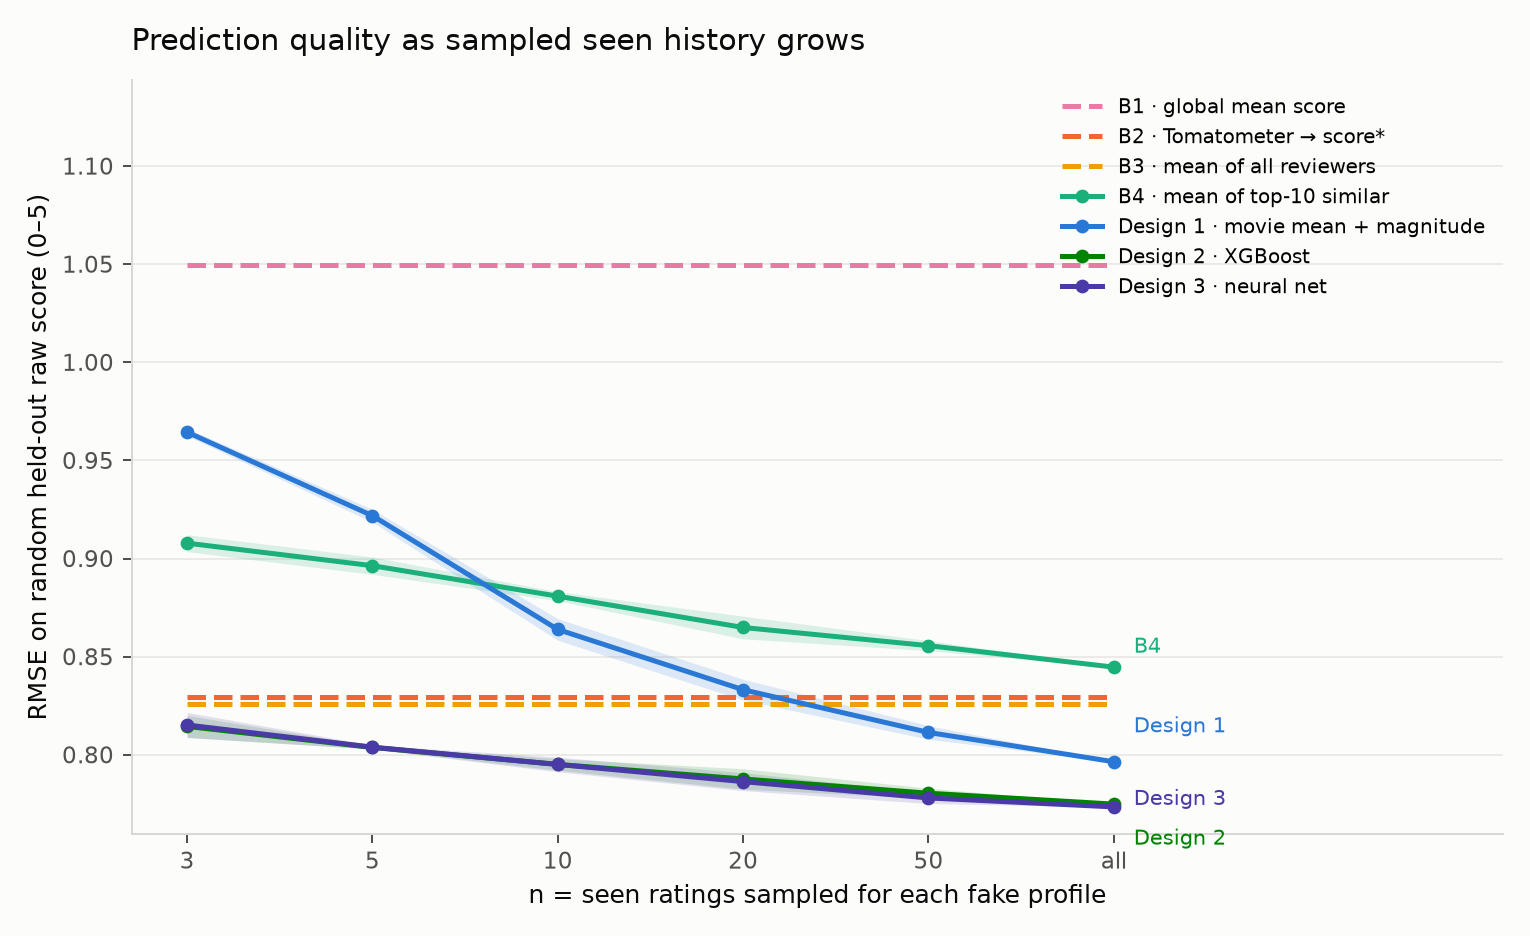
\includegraphics[width=0.92\textwidth]{plotA_rmse_vs_n.png}
\caption{Error versus sampled seen history. With paired evaluation the baselines are exactly flat; Design 1 falls smoothly from 0.964 to 0.796 and crosses them near $n=50$. Both trained models beat every baseline at every seen-count and overlap each other.}
\label{fig:plotA}
\end{figure}

Design 1 improves over B3 by 3.6\% and B2 by 4.1\% at full history, but the two trained models win everywhere: XGBoost 0.792 overall / 0.775 full history, the neural net 0.792 / 0.773. Scaling the network up --- wider (512), deeper (six residual blocks), longer training, and doubled fake-user training data --- to look for a double-descent gain moved the loss by nothing, and XGBoost itself was unchanged by the extra data: on this engineered tabular feature set the ceiling is the information in the features, not model capacity. Both models improve only gently with $n$ because their dominant feature is the movie's Tomatometer ($\approx 11\times$ the next feature in XGBoost gain), then the user's mean; this is why the learned loss is as low as it is, and it was checked to be a leakage-free calibrated consensus, not memorization.

\begin{table}[h]
\centering
\small
\begin{tabular}{lr}
\toprule
\textbf{Formula component (full-history episodes)} & \textbf{RMSE} \\
\midrule
Reviewer mean / movie consensus & 0.850 \\
\rowcolor{green!12}Magnitude-scaled movie consensus & \textbf{0.833} \\
Movie-centered signed similarity ($g_{u,c}=1$) & 0.867 \\
Full Design 1 formula & 0.850 \\
\bottomrule
\end{tabular}
\caption{Formula attribution: magnitude scaling supplies the whole gain over consensus.}
\label{tab:attr}
\end{table}

Magnitude matching supplies the entire improvement over the consensus; the signed similarity term adds nothing on top. As with the trained models, correlation-based taste matching contributes little --- the useful personalization is scale/level calibration. Across low, middle, and high critic-disagreement terciles, full-history gain over B2 is $+5.7/+6.2/+1.5\%$ for Design 1, $+7.5/+7.4/+5.6\%$ for XGBoost, and $+7.5/+7.4/+5.9\%$ for the neural net --- all three help in every tercile, the trained models most.

\begin{figure}[h]
\centering
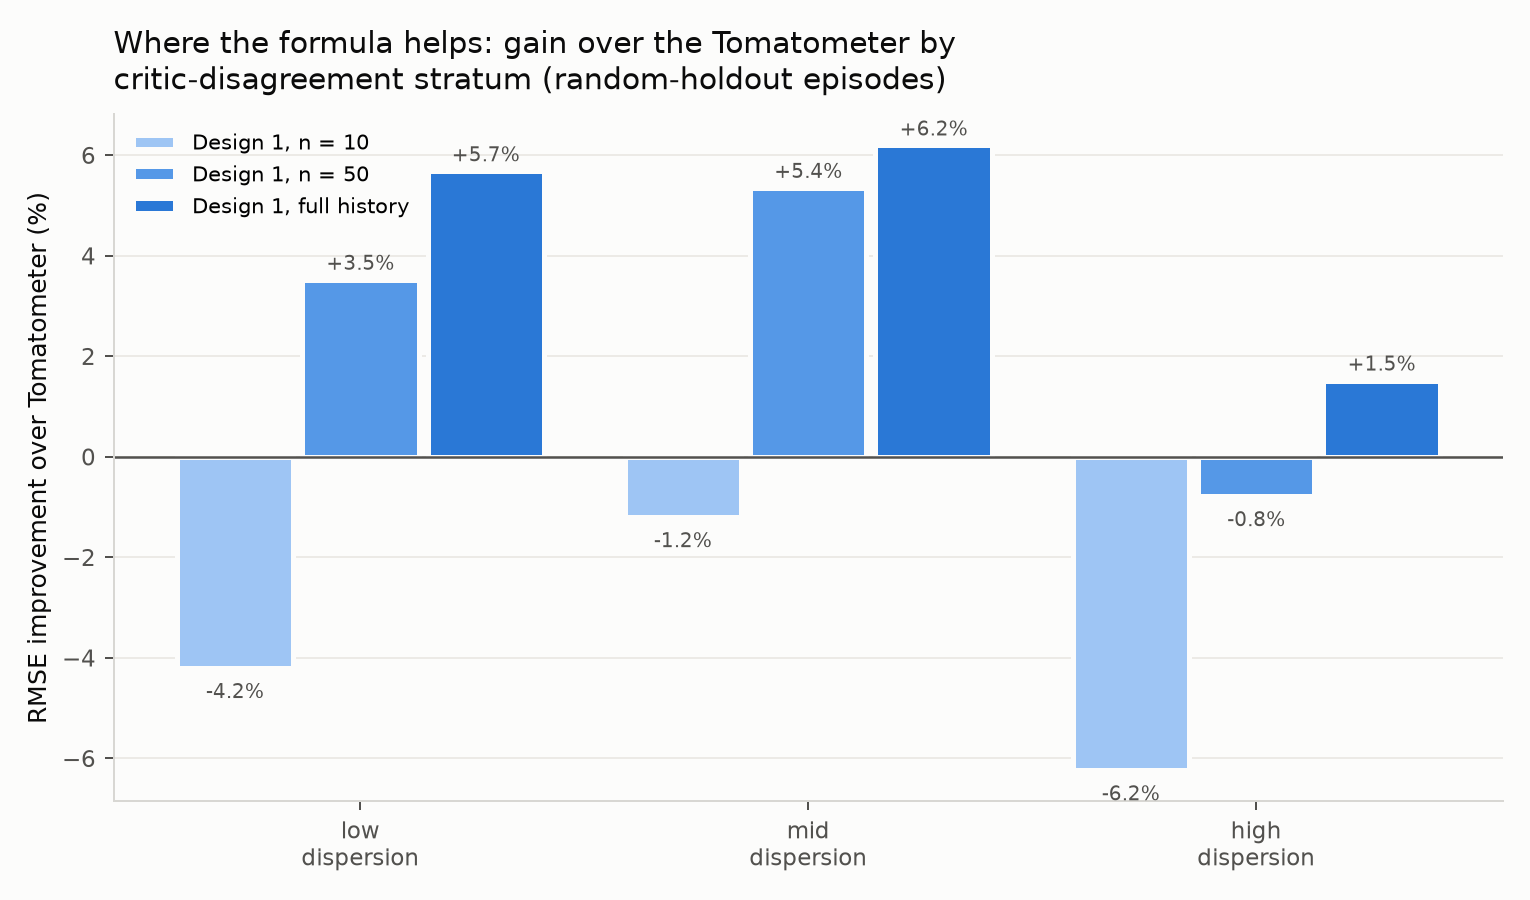
\includegraphics[width=0.86\textwidth]{plotB_gain_vs_dispersion.png}
\caption{Design 1 gain over B2 by target-movie critic disagreement.}
\label{fig:plotB}
\end{figure}

\section{Second dataset: Letterboxd community ratings}
\label{sec:letterboxd}

To test whether real, dense per-user rating histories beat the sparse critic pseudo-users above, we built a fully parallel second project on Letterboxd community ratings (Kaggle, \textasciitilde11.08M ratings), isolated in its own directory tree (\texttt{src/letterboxd/}, \texttt{data/letterboxd/}, \texttt{results/letterboxd/}) that never shares data, models, or code with the Rotten Tomatoes project. The export yields 7{,}420 members with at least five rated films across 286{,}069 films --- 11{,}078{,}045 ratings total, not 11 million distinct members. Ratings are native on a 1--10 scale (no score parsing). All three designs adopt the \emph{same} 37-feature similarity-decile contract as Design 2/3 above, minus the Tomatometer feature (Letterboxd has no critic-consensus meter): ten deciles of similarity-weighted deviation, plus seen count, overlap statistics, rater count, dispersion, genre, and the member's own mean. Design 3 is a genuinely trained residual MLP ensemble, identical in architecture to the Rotten Tomatoes network, and --- being inductive over engineered features rather than a member/movie embedding --- it scores a brand-new member's live ratings in the browser, just like Designs 1 and 2.

\begin{table}[h]
\centering
\small
\begin{tabular}{lrrrrrr}
\toprule
\textbf{Seen ratings $n$} & 3 & 5 & 10 & 20 & 50 & all \\
\midrule
B1 global mean & 2.108 & 2.108 & 2.108 & 2.108 & 2.108 & 2.108 \\
B3 mean of all members & 1.639 & 1.639 & 1.639 & 1.639 & 1.639 & 1.639 \\
B4 top-10 similar mean & 1.705 & 1.686 & 1.671 & 1.653 & 1.657 & 1.622 \\
Design 1 analytic & 1.765 & 1.670 & 1.597 & 1.561 & 1.545 & \textbf{1.507} \\
Design 2 XGBoost & 1.662 & 1.612 & 1.594 & 1.569 & 1.536 & \textbf{1.502} \\
Design 3 neural net & 1.672 & 1.621 & 1.596 & 1.562 & 1.545 & \textbf{1.518} \\
\bottomrule
\end{tabular}
\caption{Letterboxd RMSE (1--10 scale) on the same paired, nested seen-history protocol as Table~\ref{tab:nsweep}: 300 deterministic test members, 8 fixed targets each, 3 seen-order redraws.}
\label{tab:lb-nsweep}
\end{table}

\begin{figure}[h]
\centering
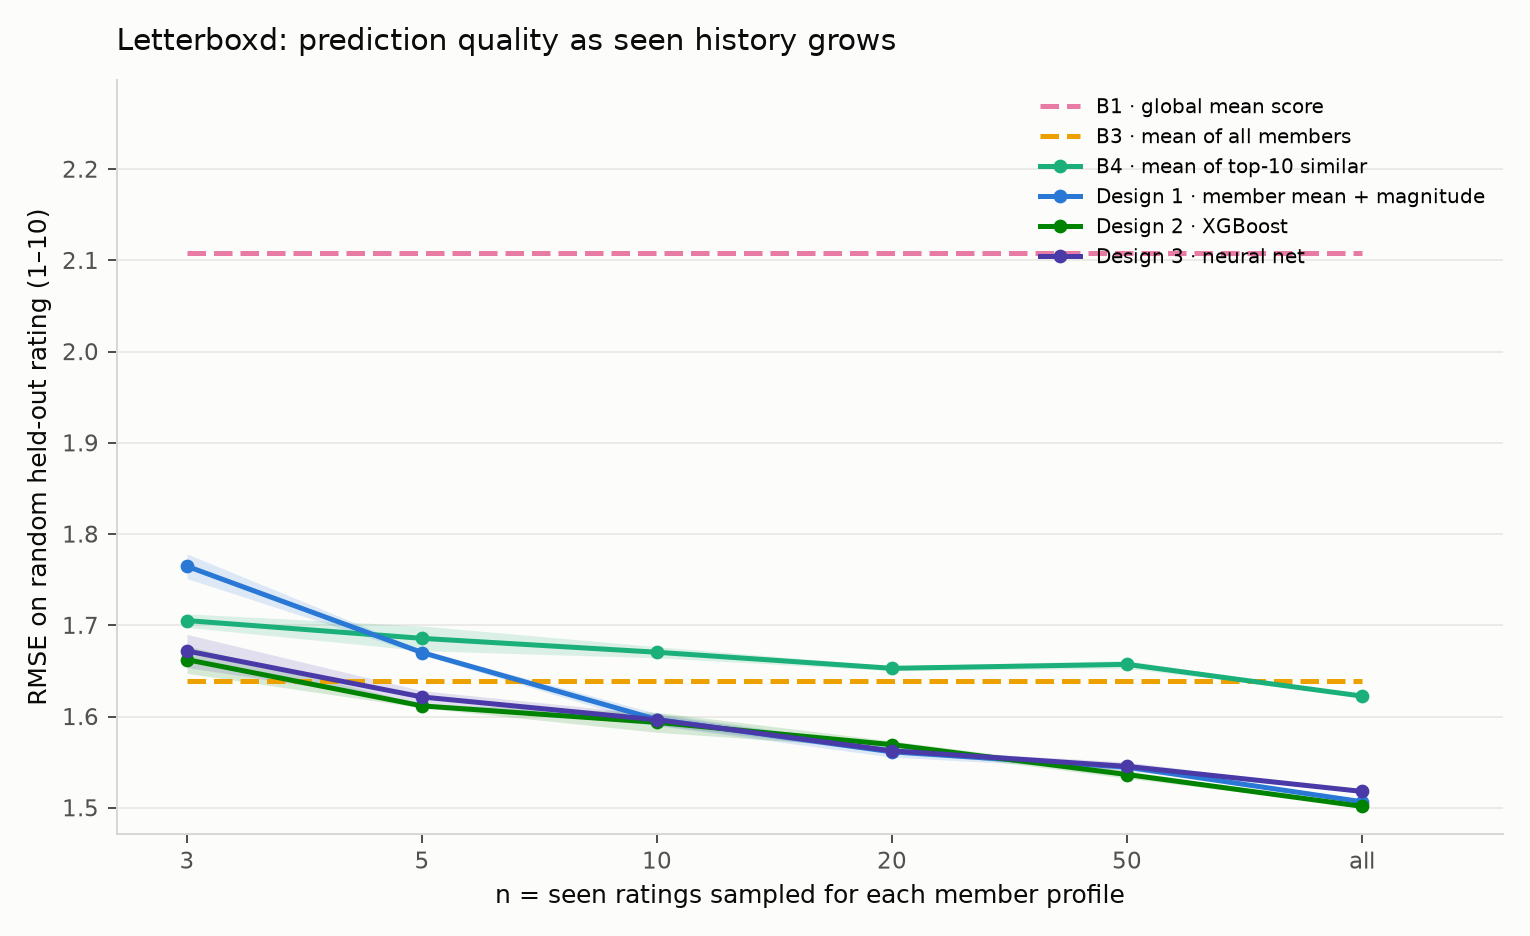
\includegraphics[width=0.92\textwidth]{../results/letterboxd/figures/plotA_rmse_vs_n.png}
\caption{Letterboxd: error versus sampled seen history, styled identically to Figure~\ref{fig:plotA}. All three designs converge to $\approx 1.50$--$1.52$ at full history.}
\label{fig:lb-plotA}
\end{figure}

\textbf{Honest cross-dataset finding.} Raw RMSE is not comparable across the two projects because the target scales differ (0--5 versus 1--10); normalizing by rating range (RMSE~/~(max$-$min)) puts them on the same footing. Rotten Tomatoes' normalized RMSE is 0.159 / 0.155 / 0.155 (Design 1/2/3); Letterboxd's is 0.167 / 0.167 / 0.169. The two are \emph{comparable}, with Rotten Tomatoes marginally \emph{better} normalized despite training on far sparser critic pseudo-user profiles instead of Letterboxd's dense real member histories. This is reported as found: more (real) rating data did not translate into a lower normalized error at this scale and with this feature contract. Letterboxd's genuine value is dense, real per-member histories rather than synthetic pseudo-users --- not a lower headline RMSE. Full numbers are in \texttt{results/letterboxd/cross\_dataset\_comparison.csv}.

\section{Isolating scale: the z-score track}
\label{sec:zscore}

The gain above is mostly calibration --- knowing a rater's own level and the movie's consensus level --- rather than similarity-based taste-matching. To test that claim directly rather than infer it, both projects also train a parallel z-score variant of every design: each rater (fake user or real member) is standardized to their own scale using \emph{seen-set} statistics for the user side and \emph{all-time} statistics for the peer side (\S\ref{sec:data} defines $z_{c,i}$ for the peer side; the user side uses the mean/std of only the ratings sampled for that episode, since a real visitor only ever has their own seen films to standardize by). The model predicts pure deviation, not level, and every prediction is converted back to the raw scale ($\hat r = \mu_{\text{user}} + \sigma_{\text{user}}\hat z$, clipped) before scoring, so raw-track and z-track RMSE are directly comparable.

\begin{table}[h]
\centering
\small
\begin{tabular}{lrrr}
\toprule
\textbf{Design} & \textbf{raw RMSE} & \textbf{z RMSE (converted back)} & \textbf{z $-$ raw} \\
\midrule
\multicolumn{4}{l}{\emph{Rotten Tomatoes (0--5)}} \\
Design 1 analytic & 0.796 & 0.926 & $+$0.130 \\
Design 2 XGBoost & 0.775 & 0.783 & $+$0.008 \\
Design 3 neural net & 0.773 & 0.788 & $+$0.015 \\
\multicolumn{4}{l}{\emph{Letterboxd (1--10)}} \\
Design 1 analytic & 1.507 & 1.640 & $+$0.134 \\
Design 2 XGBoost & 1.502 & 1.491 & $-$0.010 \\
Design 3 neural net & 1.518 & 1.497 & $-$0.021 \\
\bottomrule
\end{tabular}
\caption{Full-history RMSE, raw vs.\ z-score track, both reported on the raw scale (\texttt{results/\{rotten\_tomatoes,letterboxd\}/raw\_vs\_z.csv}).}
\label{tab:rawvsz}
\end{table}

\begin{figure}[h]
\centering
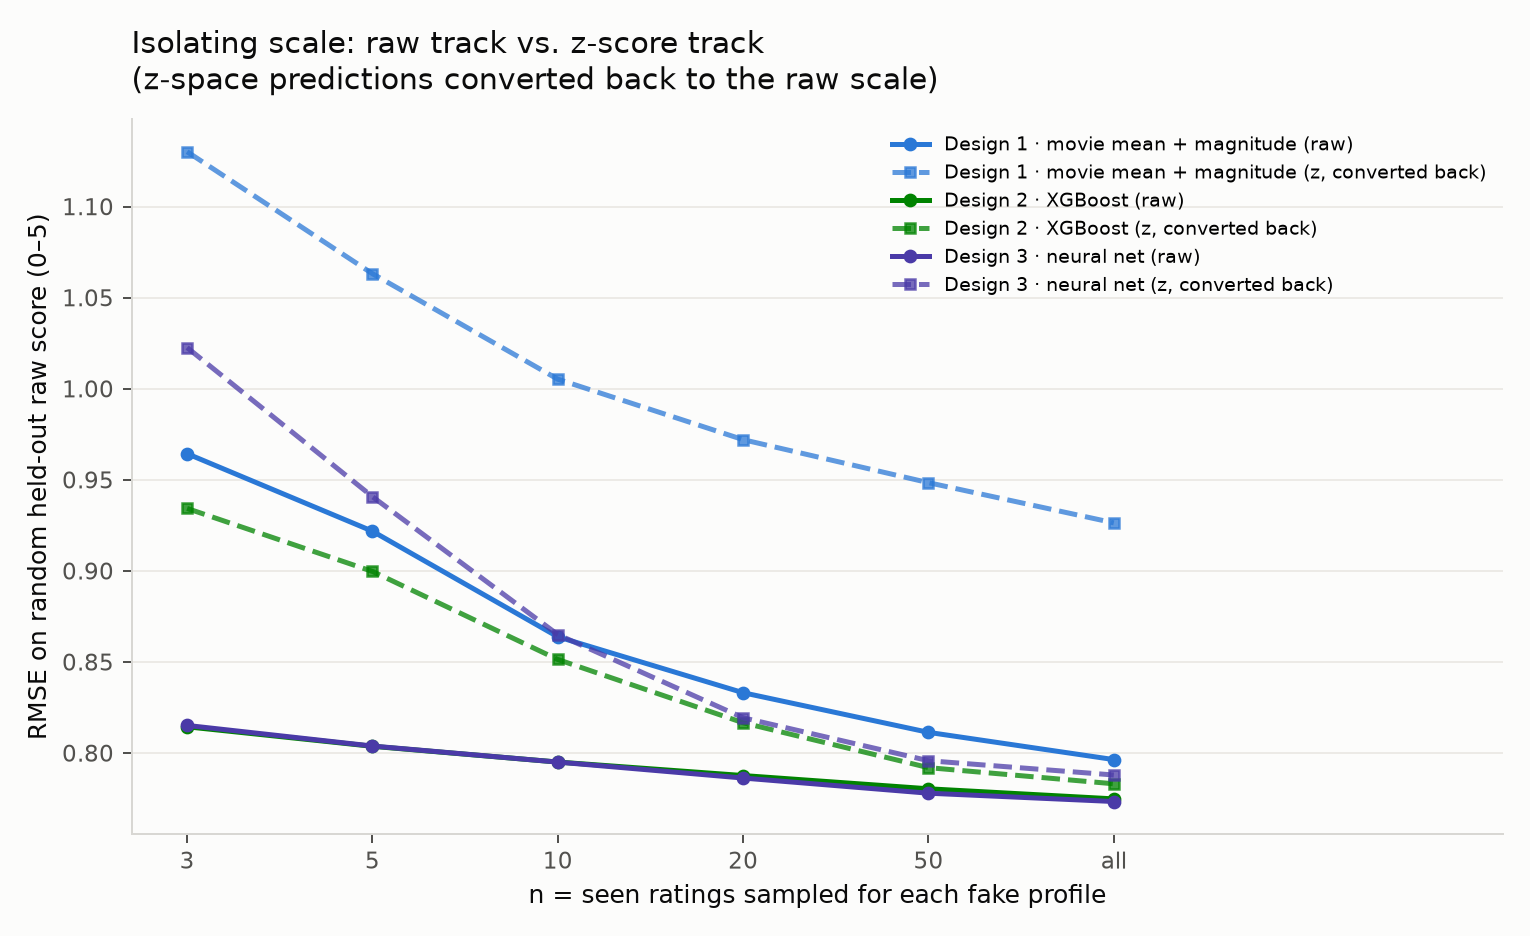
\includegraphics[width=0.92\textwidth]{plotC_raw_vs_z.png}
\caption{Rotten Tomatoes: raw (solid) vs.\ z-score (dashed) RMSE by seen count, per design.}
\label{fig:plotC}
\end{figure}

The result is \textbf{not uniform} across the two datasets, and is reported as found rather than presupposed. On Rotten Tomatoes the z-track trails the raw track at every design and every seen-count; removing the Tomatometer-anchored level signal costs more than the deviation-only target gains. On Letterboxd, the trained models (Design 2/3) come out \emph{slightly better} in z-space at full history, while the analytic formula --- which has no learned capacity to reallocate --- is worse, same as Rotten Tomatoes. A plausible reading: with a dense, purely relational feature contract (no external consensus feature like the Tomatometer) and a trained model with spare capacity, removing each rater's own level lets that capacity concentrate on the deviation signal instead of re-deriving it; the analytic formula never had spare capacity to reallocate, so it only loses the calibration information without ever regaining it. Either way, the original conclusion stands: even where the z-track modestly *helps* (Letterboxd's trained models), the gain over raw is under 1.5\%, an order of magnitude smaller than what raw calibration bought over the flat baselines in Table~\ref{tab:nsweep} --- calibration, not taste-matching, remains the dominant effect in this data.

\section{Application and limitations}

The website (Table~\ref{tab:funnel}: 1{,}000 catalog movies, 3{,}387 critics) is organized in three sections, and a sort control orders the search lists alphabetically (default), by year, or by most reviewed; the search dropdown scrolls through every match rather than truncating. \emph{(1) Films you have seen}: a search box adds a film to a table where each row carries a five-star widget --- click a star and it and all before it light gold, with the rating shown beside it --- and the search box clears after each add so films accumulate; rows can be removed. \emph{(2) Films to predict}: the same searchable star-table, but scoring is optional. \emph{(3) Predictions}: for every target film the app shows all three model predictions side by side with the movie's consensus mean and its Tomatometer. When the visitor scores some target films, the app reports the mean squared error of each method --- and of the consensus mean --- \emph{against the visitor's own score}, and marks the closest, answering ``which method predicts me best?''. Predictions update live as stars change. A dataset switcher swaps to the Letterboxd project, which is otherwise identical apart from a 1--10 numeric stepper in place of the five-star widget and no Tomatometer column.

Two secondary metrics (\texttt{comparison.analysis}, \texttt{secondary\_metrics.csv}) check that the gain is calibration rather than reordering: within-user Spearman rank correlation between predictions and held-out ratings, and precision@10 (the fraction of a pseudo-user's predicted top-10 targets that are also in their true top-10 held-out targets). Design 1's within-user Spearman is 0.578 versus 0.580 for the reviewer mean (B3) --- ranking is barely changed, consistent with the attribution finding that the win is calibration, not reordering a user's films.

Item holdout is not temporal forecasting. Lowering the critic floor to 10 adds noisier low-volume critics. The magnitude multiplier is an unregularized through-origin slope. The neural net matches but does not beat the trees here. Scores are quantized to six levels, pseudo-users are professional critics rather than casual users, and Tomatometer values are current snapshots.

\subsection*{Repository layout}

Each Rotten Tomatoes design lives in its own package under \texttt{src/rotten\_tomatoes/}: \texttt{design1\_analytic/} (\texttt{analytic.py} the formula and top-$k$ baseline, \texttt{run.py} the k-sweep and paired test, \texttt{attribution.py} the formula-component decomposition, \texttt{predict.py} app inference), \texttt{design2\_xgboost/train.py} (XGBoost training and paired-test evaluation), \texttt{design3\_neural/} (\texttt{network.py} the residual MLP, \texttt{train.py} ensemble training), and \texttt{comparison/analysis.py} (the figures and tables above). The pseudo-user substrate (\texttt{pseudo\_users.py}) and the shared 37/38-feature contract (\texttt{features.py}) live once at the \texttt{rotten\_tomatoes} package root and are imported by all three designs, so the comparison is exact by construction rather than by convention. \texttt{preprocessing/} ingests and standardizes the raw Kaggle export; \texttt{app\_catalog/} and \texttt{web\_export/} build the 1{,}000-film browser catalog and the client-side model export. \texttt{src/letterboxd/} mirrors this layout exactly (its own \texttt{features.py}, \texttt{train\_xgboost.py}, \texttt{train\_neural.py}, \texttt{analyze.py}, \texttt{web\_export.py}), sharing no code, data, or model artifacts with the Rotten Tomatoes package. \texttt{tests/} covers the formula, the random-holdout and paired-episode protocols, partition disjointness, and the feature contract.

Verified in this workspace: unit tests confirm $g_{u,c}=1.25$ for an exact $r_u=1.25\,r_c$ overlap and the specified numerator/denominator; random-holdout tests prove a sampled target is never in its own seen set; a paired-episode test proves nested seen sets are prefix-nested and deterministic; partition tests prove train/validation/test pseudo-user identities are disjoint and exhaustive; and every design, the attribution script, and the analysis/export pipeline ran end to end from the all-time processed data, with the low XGBoost loss checked to be a leakage-free calibrated consensus (flat per-$n$ baselines, a dominant Tomatometer feature, leave-one-out peer means) rather than memorization.

\vspace{0.4em}
\hrule
\vspace{0.4em}
{\small\textbf{Reproducibility.} Python, pandas, scipy.sparse, NumPy, XGBoost, PyTorch, and matplotlib. The pseudo-user substrate and feature code are shared, seeded modules (see Repository layout above), so the cross-design comparison is exact. The Letterboxd project under \texttt{src/letterboxd/} mirrors this layout exactly. Both projects also run entirely client-side in the browser (Vite/React/TypeScript, \texttt{web/}), hosted as a static GitHub Pages site with no server. Run the ordered module pipelines listed in the README from \texttt{src/}; all random seeds are fixed.}

\end{document}